% výběr jazyka
Jako jazyk pro programování měřící stanice jsem zvolil \gls{go}. Jedna z mnoha výhod je snadná \gls{cross-kompilace}, 
která mi umožňuje kompilovat programy na svém počítači a do stanice nahrávat už jen binární kód. Čemuž pomáhá i to, že 
překladač implicitně \glslink{linkovani}{linkuje} staticky.

% koncepce programu
Průběh programu, který provádí měření, vypadá takto.

% graf
\begin{figure}[H]
    \centering
    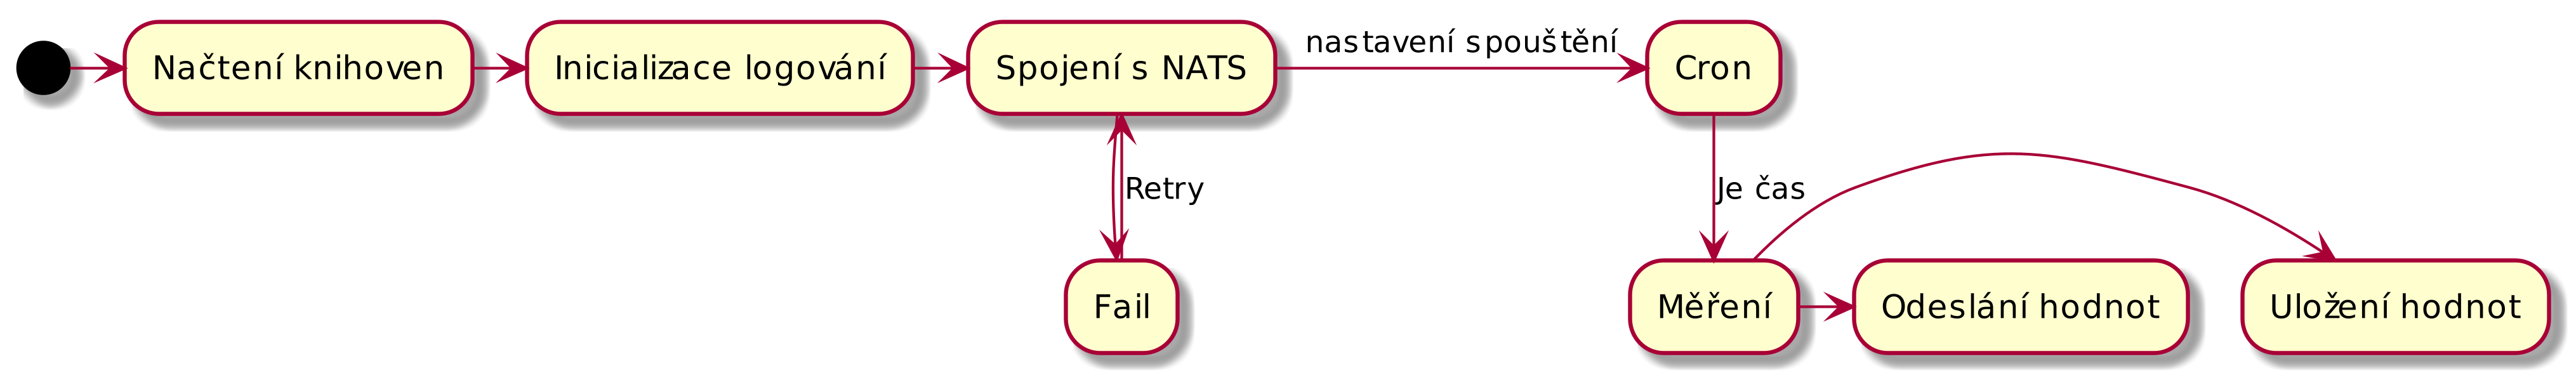
\includegraphics[width=\textwidth]{mereni.png}
    \caption{Průběh programu}
\end{figure}

Na začátku importuji šest \glslink{knihovna}{knihoven}, konkrétně používám části standardní \glslink{knihovna}{knihovny} 
pro práci s časem a operačním systémem, \glslink{knihovna}{knihovnu} pro práci s periferiemi a dále to jsou 
\glslink{knihovna}{knihovny} pro spojení s bránou, umožnění automatického spouštění programů v daný čas a logování. Ve 
funkci main jako první nastavím \glslink{knihovna}{knihovnu} logrus, která mi zajišťuje logování, nastavuji co chci 
logovat, kam to má zapsat a jak to má zformátovat. Poté otevřu spojení s bránou, inicializuji 
\glslink{knihovna}{knihovnu} na použití periferií a nastavím cron, aby mi spustil měření každých 15 minut. Nakonec je 
takový trik, jehož jediným účelem je, aby hlavní \gls{gorutina} neskončila, jedná se o čtení z kanálu do kterého, však 
nikdy nic nezapíši. A jelikož jde o blokující operaci, program nikdy neskončí.

% měření
\paragraph*{Měření}
Samotné získávání dat je velmi jednoduché. Každých 15 minut Cron zavolá funkci getMeasure(),která postupně projde přes 
všechny připojené senzory, zavolá funkce, které je obsluhují, v případě chyby je zkouší zavolat vícekrát a vrátí pole 
s naměřenými hodnotami. Pro měření jsem se snažil co nejvíce využít možností, které poskytuje  \gls{knihovna} 
\gls{periphio}, takže například data vracím ve formě struktury z této knihovny a používám ji pro získávání hodnot ze 
dvou senzorů, pro třetí ji nepoužívám jen z toho důvodu, že ho zatím nepodporuje. Měření z BME280 je velmi jednoduché. 
V podstatě otevřu sběrnici, přečtu data a vrátím je, vše za použití výše zmíněné knihovny. Z DS18B20 to je velmi 
podobné, jen nemohu použít \gls{periphio}, takže používám knihovnu, jež využívá modul kernelu, který zpřístupňuje tento 
senzor přes virtuální souborový systém. Senzor DHT11 je na použití asi nejsložitější. Používám sice externí knihovnu, 
avšak ta pro přístup ke \acrshort{gpio} využívá \gls{periphio}. Jinak je měření velmi obdobné jako u ostatních čidel 
s tím rozdílem, že je velmi chybové, takže se musí vícekrát opakovat.

\paragraph*{DHT11}
S tímto senzorem jsem měl asi největší problémy. Nejenom že jsem musel laborovat s nastavením verze api knihovny 
\gls{periphio}, ale i samotná knihovna pro obsluhu senzoru obsahovala chyby. Takže jsem ji důkladně prozkoumal 
a porovnal s datasheetem(\url{https://www.mouser.com/datasheet/2/758/DHT11-Technical-Data-Sheet-Translated-Version-1143054.pdf}) 
k senzoru. Našel jsem dvě zásadní chyby. Jedna byla, že knihovna vyslala příliš krátký startovací pulz, takže ani čidlo 
neprobudila, to se dalo vyřešit jednoduše, prostě jsem do programu přidal pauzu. A druhá, že špatně zpracovávala data 
co, z čidla četla. Před úpravou mi vracela nereálné hodnoty teploty a vlhkosti, konkrétně vracela chybu, že načtená data 
jsou mimo rozsah, protože hodnoty zpracovávala jako jedno velké šestnáctibitové číslo, ale v datasheetu jsem se dočetl 
že tyto dva bajty představují číslo v desetinné čárce, ale velmi neobvykle. První bajt je celá část a druhý desetinná 
a zároveň s tím se v datasheetu píše, že rozlišovací schopnost senzoru je 1 \textdegree C a 1 \%, takže jsem druhý bajt 
zahodil a dál pracoval pouze s tím prvním. A to fungovalo na jedničku. Tuto zvláštnost s rozlišením bych asi vysvětlil 
tím, že komunikační protokol bude shodný i s dražšími senzory s lepším rozlišením, a to možná souvisí i s chybami 
v knihovně, poněvadž je určena i pro ně. Takže abych jejich podporu nerozbil jsem mé úpravy podmínil použitím správného 
typu čidla. Moje upravená verze kterou používám je k nalezení zde: \url{https://github.com/prokopparuzek/go-dht.git}.

% ukládání dat
\paragraph*{Ukládání}
Pro ukládání dat na měřící stanici jsem nevymýšlel nic složitého. Vezmu jen data z každého senzoru, přidám 
\gls{timestamp}, tím se vyhnu problémům s reprezentací času a převody časových pásem, a to vše přidám za konec souboru 
konkrétního senzoru. Data ukládám ve formátu \acrshort{csv}. Jednotlivé hodnoty/sloupce nijak neoznačuji, nechávám to na 
utilitách, jejichž cílem bude data obnovit, ty jediné s nimi takto budou pracovat a to jen občas, takže to myslím 
nevadí, a navíc to zjednodušuje kód.

\paragraph*{Message broker}
Jako základní \gls{message-broker} by se dal použít server NATS. Já použiji trochu bezpečnější variantu, konkrétně 
použiji nadstavbu nazývanou NATS-streaming. Stejně jako NATS se jedná o lehkou aplikaci napsanou v \gls{go}, takže 
zabírá minimum zdrojů \parencite{root.cz:NATS-streaming}. Já jsem ji vybral z důvodu jednoduchosti, dostupnosti široké 
škály klientských knihoven a též již zmiňované lehkosti.

% odesílání
\paragraph*{Odesílání}
Odesílání dat začíná vlastně už na úplném začátku, kdy se spojím se \glslink{brana}{bránou} a pak až do konce držím 
spojení otevřené. Samotné odeslání dat do \glslink{message-broker}{message brokera} se vlastně moc neliší od uložení. 
Taky vezmu data, přidám \gls{timestamp} a pošlu je. Je tu však pár rozdílů. Data posílám ve formátu \gls{JSON}, který je 
jednoduchý a čitelný. Z důvodu možných latencí, nedostupnosti sítě\ldots odesílám každou zprávu v samostatné 
\glslink{gorutina}{gorutině}, abych neblokoval další měření, jelikož když se zprávu nepovede odeslat, tak ji zkouším 
poslat po minutě další zhruba dvě hodiny. No a to je vše, po odeslání zprávy už nemusím nic řešit, poněvadž server si ji 
uloží a pošle dál, takže už se neztratí.
